\documentclass{article}
\usepackage{tikz}
\usetikzlibrary{shapes, shapes.multipart, positioning, fit, backgrounds, arrows.meta}
\usepackage[margin=1in]{geometry}

\begin{document}

% ==========================================
% USE CASE DIAGRAM
% ==========================================
\begin{figure}[htbp]
\centering
\vspace{1cm}
\resizebox{\textwidth}{!}{
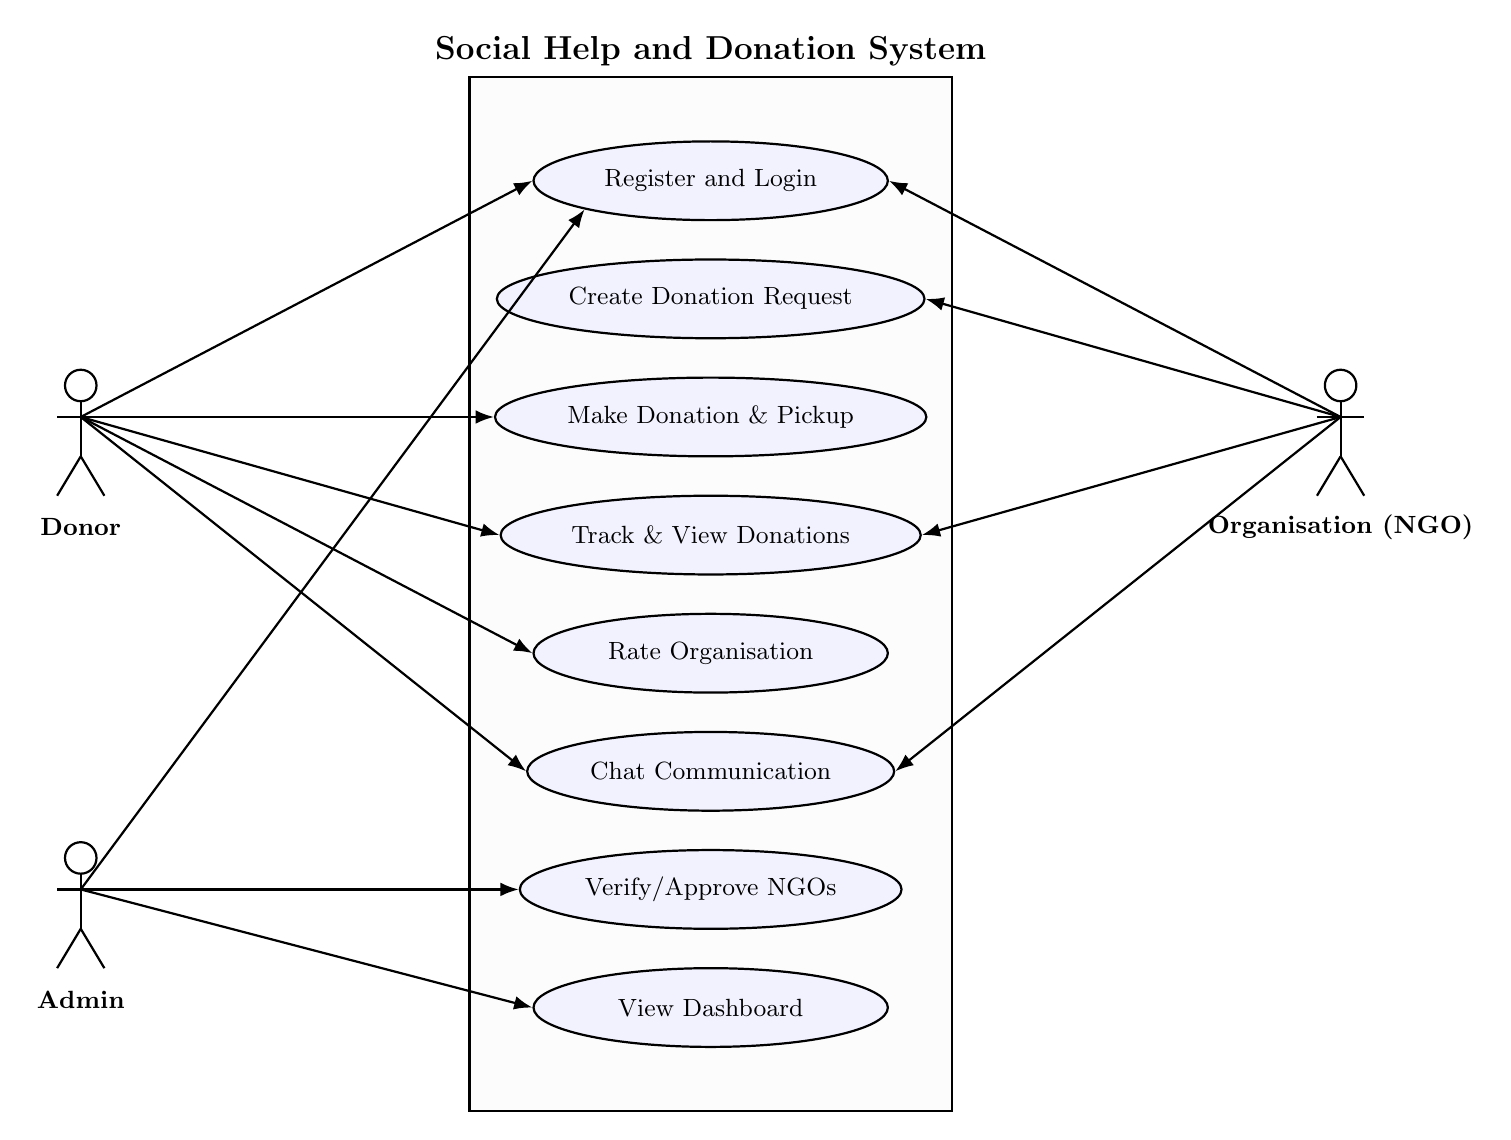
\begin{tikzpicture}[
    >=Latex, thick,
    actor/.style={align=center, font=\small\bfseries},
    usecase/.style={draw, ellipse, minimum width=4.5cm, minimum height=1cm, align=center, fill=blue!5, font=\small}
]

% Stickman Definition
\tikzset{
    stickman/.pic={
        \coordinate (-chest) at (0, 0);
        \draw[thick] (0, 0.4) circle (0.2); 
        \draw[thick] (0, 0.2) -- (0, -0.5); 
        \draw[thick] (-0.3, 0) -- (0.3, 0); 
        \draw[thick] (0, -0.5) -- (-0.3, -1); 
        \draw[thick] (0, -0.5) -- (0.3, -1); 
    }
}

\node[usecase] (UC1) at (0, 8.5) {Register and Login};
\node[usecase] (UC2) at (0, 7) {Create Donation Request};
\node[usecase] (UC3) at (0, 5.5) {Make Donation \& Pickup};
\node[usecase] (UC4) at (0, 4) {Track \& View Donations};
\node[usecase] (UC5) at (0, 2.5) {Rate Organisation};
\node[usecase] (UC6) at (0, 1) {Chat Communication};
\node[usecase] (UC7) at (0, -0.5) {Verify/Approve NGOs};
\node[usecase] (UC8) at (0, -2) {View Dashboard};

\begin{scope}[on background layer]
    \node[draw, rectangle, thick, fill=gray!2, inner sep=0.8cm, fit=(UC1) (UC8)] (System) {};
    \node[anchor=south, font=\large\bfseries] at (System.north) {Social Help and Donation System};
\end{scope}

\pic (DonorPic) at (-8, 5.5) {stickman};
\node[actor] (DonorLabel) at (-8, 4.1) {Donor};

\pic (OrgPic) at (8, 5.5) {stickman};
\node[actor] (OrgLabel) at (8, 4.1) {Organisation (NGO)};

\pic (AdminPic) at (-8, -0.5) {stickman};
\node[actor] (AdminLabel) at (-8, -1.9) {Admin};

\draw[->] (DonorPic-chest) -- (UC1.west);
\draw[->] (DonorPic-chest) -- (UC3.west);
\draw[->] (DonorPic-chest) -- (UC4.west);
\draw[->] (DonorPic-chest) -- (UC5.west);
\draw[->] (DonorPic-chest) -- (UC6.west);

\draw[->] (OrgPic-chest) -- (UC1.east);
\draw[->] (OrgPic-chest) -- (UC2.east);
\draw[->] (OrgPic-chest) -- (UC4.east);
\draw[->] (OrgPic-chest) -- (UC6.east);

\draw[->] (AdminPic-chest) -- (UC1.south west); 
\draw[->] (AdminPic-chest) -- (UC7.west);
\draw[->] (AdminPic-chest) -- (UC8.west);

\end{tikzpicture}
}
\end{figure}

\newpage

% ==========================================
% CLASS DIAGRAM
% ==========================================
\begin{figure}[htbp]
\centering
\resizebox{\textwidth}{!}{
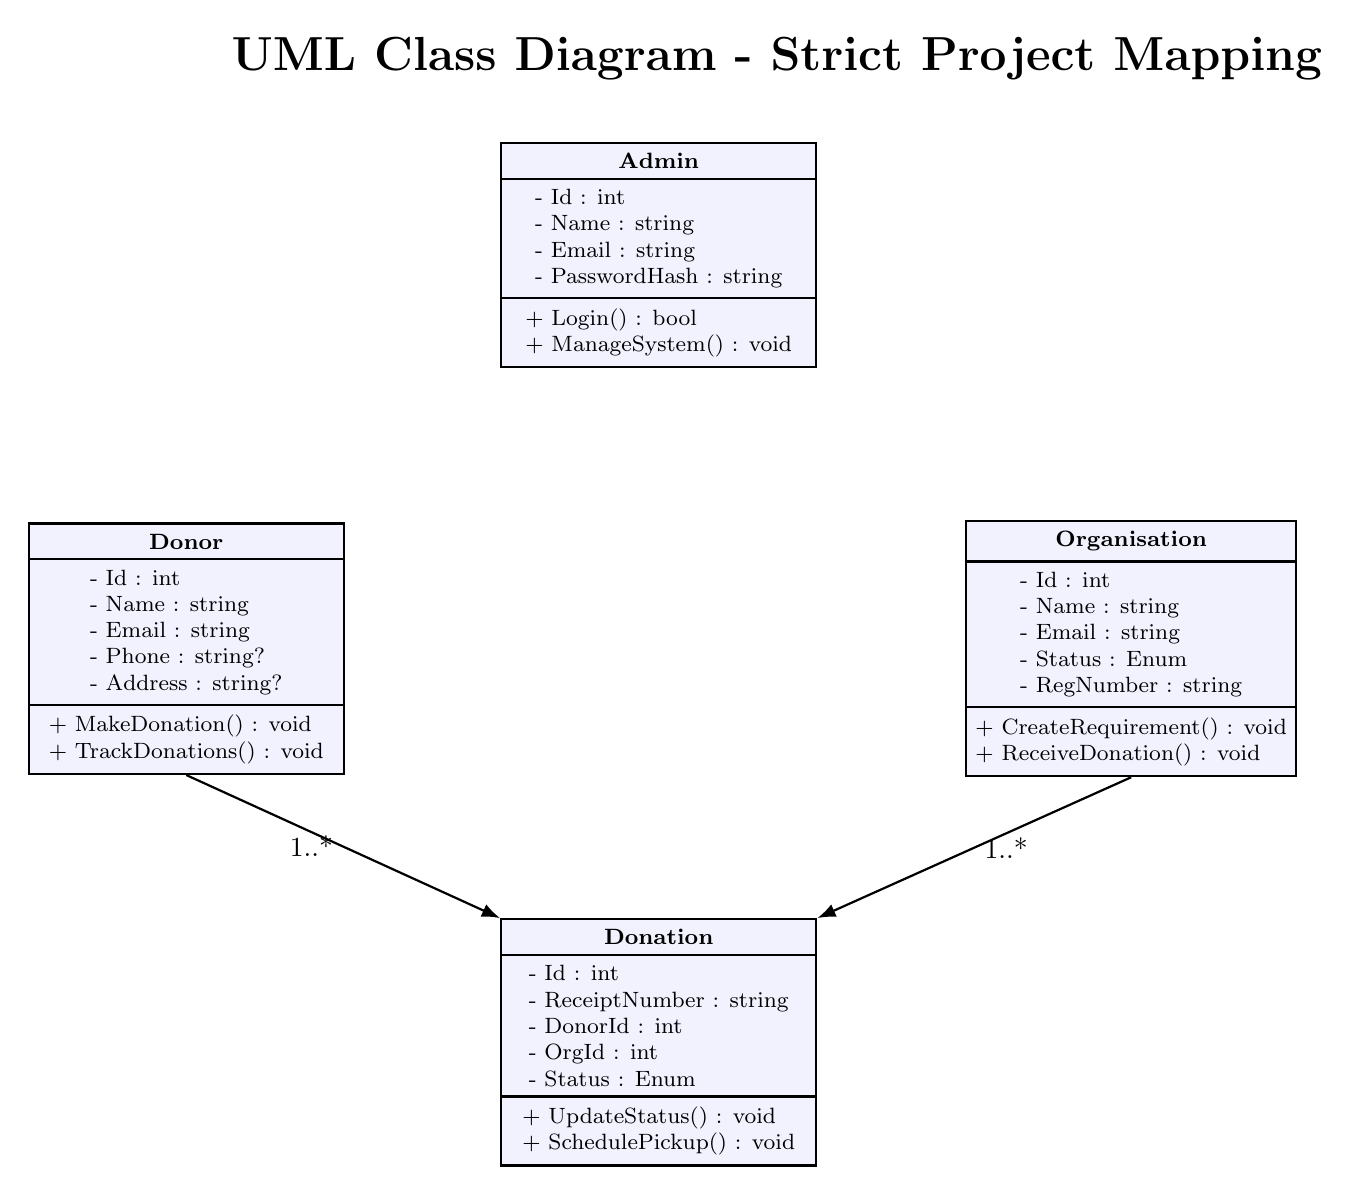
\begin{tikzpicture}[
    >=Latex,
    class/.style={
        draw, rectangle split, rectangle split parts=3,
        minimum width=4cm, align=left, fill=blue!5, thick, font=\footnotesize
    }
]

\node[font=\LARGE\bfseries, align=center] at (1.5, 9.5) {UML Class Diagram - Strict Project Mapping};

\node[class] (Admin) at (0, 7) {
    \textbf{Admin}
    \nodepart{second}
    - Id : int \\
    - Name : string \\
    - Email : string \\
    - PasswordHash : string 
    \nodepart{third}
    + Login() : bool \\
    + ManageSystem() : void
};

\node[class] (Donor) at (-6, 2) {
    \textbf{Donor}
    \nodepart{second}
    - Id : int \\
    - Name : string \\
    - Email : string \\
    - Phone : string? \\
    - Address : string?
    \nodepart{third}
    + MakeDonation() : void \\
    + TrackDonations() : void
};

\node[class] (Org) at (6, 2) {
    \textbf{Organisation}
    \nodepart{second}
    - Id : int \\
    - Name : string \\
    - Email : string \\
    - Status : Enum \\
    - RegNumber : string
    \nodepart{third}
    + CreateRequirement() : void \\
    + ReceiveDonation() : void
};

\node[class] (Donation) at (0, -3) {
    \textbf{Donation}
    \nodepart{second}
    - Id : int \\
    - ReceiptNumber : string \\
    - DonorId : int \\
    - OrgId : int \\
    - Status : Enum
    \nodepart{third}
    + UpdateStatus() : void \\
    + SchedulePickup() : void
};

\draw[->, thick] (Donor.south) -- (Donation.north west) node[midway, left] {1..*};
\draw[->, thick] (Org.south) -- (Donation.north east) node[midway, right] {1..*};

\end{tikzpicture}
}
\end{figure}

\end{document}
